\subsection{Nuclear Transparency}

\begin{equation}
    T(Q^2) = \frac{\int_{V} d^{3} p_{m} d E_{m} Y_{exp }(E_{m}, \vec{p}_{m})}
                  {\int_{V} d^{3} p_{m} d E_{m} Y_{PWIA}(E_{m}, \vec{p}_{m})}
\end{equation}


% TODO: replace this with a pdf
\begin{figure}[!h]
    \centering
    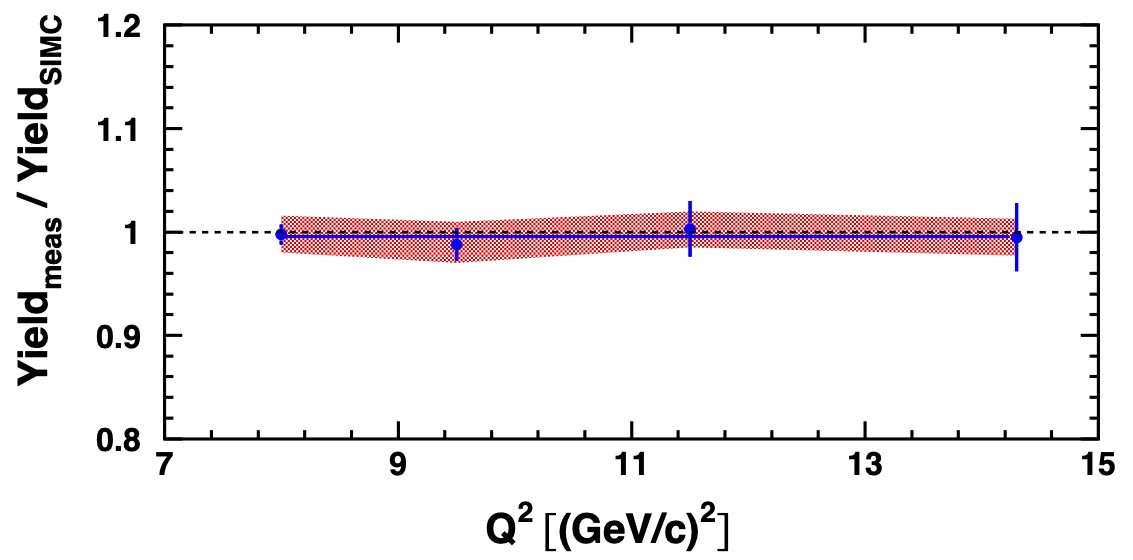
\includegraphics[width=0.8\textwidth]{chap5/lh2_results.png}
    \caption{
            Nuclear transparency for ${}^{1}H(e,e'p)$ as a function of
            momentum transfer.
            The error bars represent statistical uncertainty and the
            shaded band represents the 4.0\% systematic uncertainty.
            }
    \label{fig:lh2_transparency_results}
\end{figure}



\begin{figure}[!h]
    \centering
    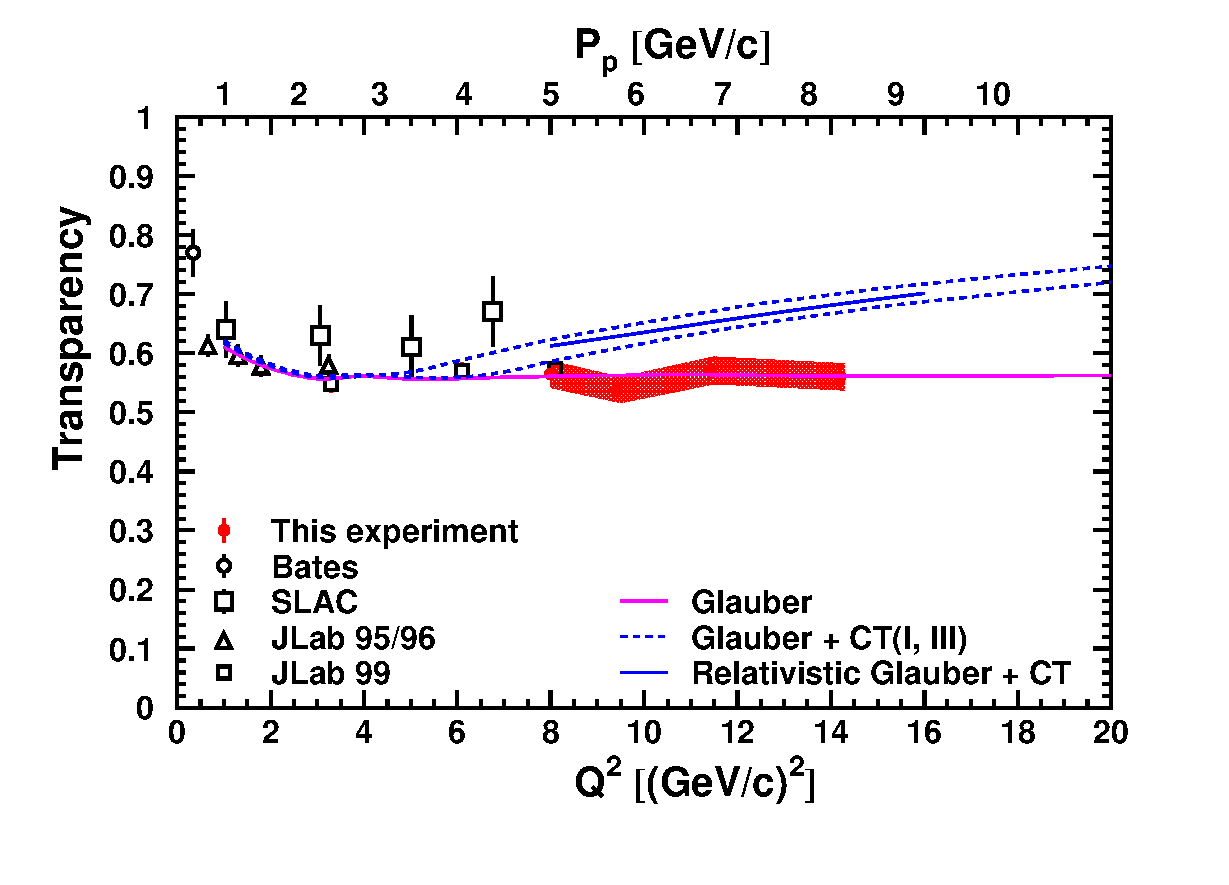
\includegraphics[width=0.8\textwidth]{chap5/c12_results.pdf}
    \caption{
            Nuclear transparency for ${}^{12}C(e,e'p)$ as a function of
            momentum transfer.
            The results of this experiment, E12-06-107, are shown in red along
            with previous measurements in open shapes.
            The error bars represent statistical uncertainty and the
            shaded band represents the 4.0\% systematic uncertainty.
            The magenta line is the prediction of a Glauber
            model that does not include CT~\cite{Pandharipande_1992}.
            The dashed lines represent predictions, for two choices of
            parameters, of a model including CT~\cite{Frankfurt_1995}.
            The solid line represents the prediction of a relativistic Glauber
            model that includes CT~\cite{Cosyn_2006}.
            }
    \label{fig:c12_transparency_results}
\end{figure}


